\documentclass{zkdl-presentation-template}

\usepackage[T1]{fontenc}
\usepackage{kerkis}
\usepackage{kmath}
\usepackage{bbm}
%\usepackage{concmath}
\usepackage{centernot}
\usepackage{mdframed}

\newcommand\leftarrowS{\leftarrow\joinrel\smalldollar}
\newcommand\rightarrowS{\smalldollar\joinrel\rightarrow}

\makeatletter
\newcommand{\smalldollar}{\mathrel{\mathpalette\small@dollar\relax}}
\newcommand{\small@dollar}[2]{%
  \vcenter{\hbox{%
    $#1\textnormal{\fontsize{0.7\dimexpr\f@size pt}{0}\selectfont\$}$%
  }}%
}
\makeatother

\tikzset{
    grid_cell/.style={
        rectangle, 
        draw=black, 
        very thick,
        minimum size=0.75cm, 
        font=\large\bfseries
    },
    grid_label/.style={
        font=\small
    },
    hypercube_highlight/.style={
        fill=gray!40
    }
}

\title[UltraGroth]{\textbf{UltraGroth. Lookup Checks Enabled in Groth16}}
\author{Distributed Lab}
\date{September 4, 2025}
\homepage{zkdl-camp.github.io}
\github{ZKDL-Camp}

\begin{document}
    \frame {
        \tikz [remember picture,overlay]
        \node at
            ([yshift=1.5cm,xshift=-1.5cm]current page.south east) 
            %or: (current page.center)
            {
\includegraphics[width=60pt]{images/logo.png}};
        \titlepage
    }

	\section{Introduction}

    \begin{frame}{Motivation}
        We typically want to check \textbf{inclusion $\{z_i\}_{i \in [n]} \subseteq
        \{t_j\}_{j \in [v]}$}, where $\{z_i\}_{i \in [n]}$ is part of the witness
        while $\{t_j\}_{j \in [v]}$ is the lookup table.

        \textcolor{green!60!black}{\textbf{Example usage:}} effective range-checks 
        (Bionetta, Rarimo circuits, non-native ZK verifications etc.)


        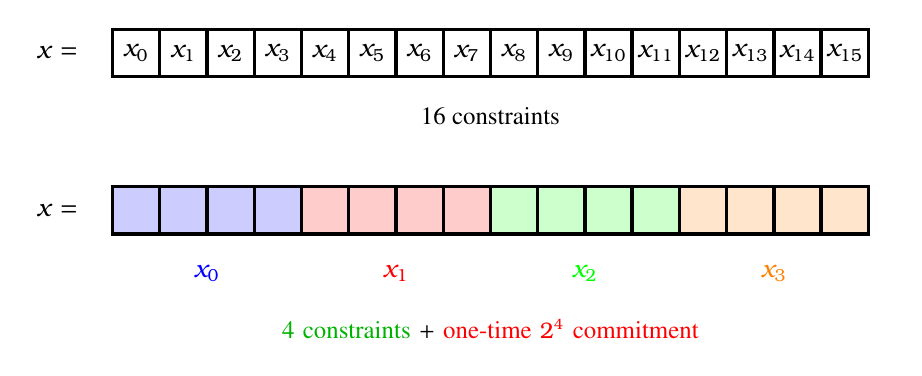
\begin{tikzpicture}[
            % Style for the bit squares, now smaller
            bit/.style={draw, very thick, minimum size=0.6cm, outer sep=0},
            % Style for the labels below the rows
            info/.style={font=\small}
        ]

        % --- First line: 16 individual bits ---
        \node at (-1, 2.0) {$x=$};
        % Draw the 16 squares and labels separately to ensure constant box size
        \foreach \i in {0,...,15} {
            % Draw the box first
            \node[bit] at (\i*0.6, 2.0) {};
            % Then place the label at the same coordinate
            \node at (\i*0.6, 2.0) {$x_{\i}$};
        }
        % Add the text below the row, centered
        \node[info] at (7.5*0.6, 1.2) {16 constraints};


        % --- Second line: 4 chunks of 4 bits ---
        \node at (-1, 0) {$x=$};
        % Draw the 4 highlighted chunks with different gentle colors and their labels
        \foreach \i/\chunkcolor/\textcolor in {0/blue!20/blue, 1/red!20/red, 2/green!20/green, 3/orange!20/orange} {
            % Draw the colored rectangle for the chunk
            \fill[\chunkcolor] (\i*4*0.6 - 0.3, -0.3) rectangle (\i*4*0.6 + 4*0.6 - 0.3, 0.3);
            % Add the chunk label below with corresponding color
            \node[text=\textcolor, font=\bfseries] at (\i*4*0.6 + 1.5*0.6, -0.8) {$x_{\i}$};
        }
        % Draw the 16 squares on top (without labels)
        \foreach \i in {0,...,15} {
            \node[bit] at (\i*0.6, 0) {};
        }
        % Draw vertical lines to separate the chunks
        \foreach \i in {1,2,3} {
            \draw[thick] (\i*4*0.6 - 0.3, -0.3) -- (\i*4*0.6 - 0.3, 0.3);
        }
        % Add the text below the row, centered
        \node[info, text width=10cm, align=center] at (7.5*0.6, -1.5) {\textcolor{green!70!black}{4 constraints} + \textcolor{red}{one-time $2^4$ commitment}};

        \end{tikzpicture}

        \textbf{Generally:} for $n$-bit range-check, the circuit's complexity
        reduces from $\mathcal{O}(n)$ to $\mathcal{O}(2^w + \frac{n}{w})$, which
        yields $\mathcal{O}(n/\log n)$ assymptotic.
    \end{frame}

    \begin{frame}{Logup Check}
        \begin{theorem}[Some stuff from ZKDL Camp]
            The inclusion check $\{z_i\}_{i \in [n]} \subseteq \{t_i\}_{i \in
            [v]}$ is satisfied if and only if there exists the set of
            multiplicities $\{\mu_i\}_{i \in [v]}$ where $\mu_i = \#\{j \in [n]:
            z_j = t_i\}$ such that for $\gamma \leftarrowS \mathbb{F}$:
            \begin{equation*}
                \sum_{i \in [n]} \frac{1}{\gamma + z_i} = \sum_{i \in [v]} \frac{\mu_i}{\gamma + t_i}
            \end{equation*}
        \end{theorem}

        \textit{Naive approach:} Define \texttt{\textcolor{blue!70!black}{signal}} \texttt{gamma} and implement this check
        in-circuit. This costs exactly $n + 2v$ constraints.

        \textcolor{red!70!black}{\textbf{Problem:}} We \textit{cannot define
        random} signals in Circom since Groth16, compared to
        $\mathcal{P}$lon$\mathcal{K}$ or sumcheck-based approaches, is not
        compiled from interactive protocol using Fiat-Shamir heuristic.
    \end{frame}

    \begin{frame}{Other implications}
        UltraGroth, though, is not about lookup checks only.

        Assume that you need to implement multiplication of two matrices $A,B
        \in \mathbb{F}^{n \times n}$. \textbf{Naive way} is to compute $C=AB$ by definition:
        \begin{equation*}
            C_{i,j} = \sum_{k=1}^n A_{i,k}B_{k,j} \hspace{30px} \textcolor{gray!80!black}{\texttt{// Costs $n$ constraints per $C_{i,j}$}}
        \end{equation*}
        As we have $n^2$ elements in $C$, we thus need $n^3$ constraints.

        We can instead apply the \textbf{Freiveld's protocol}. Sample random 
        $\boldsymbol{\gamma} \leftarrowS \mathbb{F}^n$, compute $C$ off-circuit 
        and then verify:
        \begin{equation*}
            AB\boldsymbol{\gamma} = C\boldsymbol{\gamma} \hspace{30px} \textcolor{gray!80!black}{\texttt{// Costs $3n^2$ constraints}}
        \end{equation*} 

        \textbf{Example:} Attention layer implementation in zkML.
    \end{frame}

    \begin{frame}{Plan}
        \begin{enumerate}
            \item We recap the Groth16 construction.
            \item We identify how to make it interactive.
            \item We specify how Fiat-Shamir transformation should be applied.
            \item We show how it can be practically implemented.
        \end{enumerate}
    \end{frame}

    \section{Groth16 Recap}

    \begin{frame}{R1CS}
        Recall that we can encode any NP statement in the form of $m$ equations
        of form $\langle \boldsymbol{\ell}_j, \mathbf{z} \rangle \cdot \langle
        \boldsymbol{r}_j, \mathbf{z} \rangle = \langle \boldsymbol{o}_j,
        \mathbf{z} \rangle$ for $j \in [m]$ and $\mathbf{z} \in \mathbb{F}^n$.
        Such way of representing the statement is called \textbf{R1CS
        arithmetization}.

        This equality is rewritten more succinctly in the matrix form:
        \begin{equation*}
            L\mathbf{z} \odot R\mathbf{z} = O\mathbf{z}
        \end{equation*}

        \begin{itemize}[label=\textcolor{green!70!black}{\ding{51}}]
            \item As of now, this is one of the most optimal arithmetization
            systems available (compared to PlonK and AIR).
            \item All linear operations over elements of $\mathbf{z}$ cost
            \textbf{0 constraints}, compared to PlonK.
        \end{itemize}
    \end{frame}

    \begin{frame}
        \begin{example}
    Suppose the program computes the expression $y=x_1^3 + x_2^2$. 

    % Define circle styles and colors
\colorlet{circle edge}{gray!50!black}
\colorlet{circle area}{gray!20}
\colorlet{gate1 edge}{green!50!black}
\colorlet{gate1 area}{green!20}
\colorlet{gate2 edge}{blue!50!purple}
\colorlet{gate2 area}{blue!20!white}
\colorlet{gate3 edge}{blue!50!black}
\colorlet{gate3 area}{blue!20}

\tikzset{
    var/.style={circle, draw=circle edge, fill=circle area, very thick, minimum size=1cm, text centered},
    gate1/.style={circle, draw=gate1 edge, fill=gate1 area, ultra thick, minimum size=1cm, text centered},
    gate2/.style={circle, draw=gate2 edge, fill=gate2 area, ultra thick, minimum size=1cm, text centered},
    gate3/.style={circle, draw=gate3 edge, fill=gate3 area, ultra thick, minimum size=1cm, text centered},
    arrow/.style={-Stealth, ultra thick}
}

\vspace{10px}
\begin{columns}
\begin{column}{0.45\textwidth}
\begin{center}
    \underline{\textbf{Circuit Diagram}}

        \scalebox{0.7}{
        \begin{tikzpicture}
            % Nodes
            \node[var] (x1) at (0, 1) {$x_1$};
            \node[gate2] (x1_x1) at (2, 1) {$\times$};
            \node[gate2] (x1_x1_x1) at (4, 1) {$\times$};

            \node[var] (x2) at (0, -1) {$x_2$};
            \node[gate2] (x2_x2) at (2, -1) {$\times$};

            \node[gate1] (plus) at (5.0, -0.5) {$+$};

            % x1**3
            \draw[arrow,gray] (x1) to [bend left=45] (x1_x1);
            \draw[arrow,gray] (x1) to [bend right=15] (x1_x1);
            \draw[arrow,gray] (x1_x1) -- node[midway, above] {\textcolor{blue}{$t_1$}} (x1_x1_x1);
            \draw[arrow,gray] (x1) to [bend right=45] (x1_x1_x1);

            % x2**2
            \draw[arrow,gray] (x2) to [bend left=30] (x2_x2);
            \draw[arrow,gray] (x2) to [bend right=30] (x2_x2);

            % Summation
            \draw[arrow,gray] (x1_x1_x1) -- node[midway, right] {\textcolor{green!50!black}{$t_2$}} (plus);
            \draw[arrow,gray] (x2_x2) -- node[midway, below] {\textcolor{purple}{$t_3$}} (plus);

            % Result
            \node[var] (q) at (7.0, -0.5) {$y$};
            \draw[arrow,gray!50!black] (plus) -- (q);
        \end{tikzpicture}
        }
    \end{center}
\end{column}

\begin{column}{0.4\textwidth}
    \begin{center}
        \underline{\textbf{Constraints}}
        \begin{align*}
            \textcolor{blue}{t_1} = x_1 \cdot x_1 \\
            \textcolor{green!50!black}{t_2} = \textcolor{blue}{t_1} \cdot x_1 \\
            \textcolor{purple}{t_3} = x_2 \cdot x_2 \\
            y = \textcolor{green!50!black}{t_2} + \textcolor{purple}{t_3}
        \end{align*}
    \end{center}
\end{column}
\end{columns}

\vspace{10px}

 In this case, the witness looks as $\boldsymbol{z} = (1,x_1,x_2,t_1,t_2,t_3,y)$,
and (for simplicity, consider only $L,R$):
\begin{gather*}
    \footnotesize L = \begin{bmatrix}
        0 & 1 & 0 & 0 & 0 & 0 & 0\\
        0 & 0 & 0 & 1 & 0 & 0 & 0 \\
        0 & 0 & 1 & 0 & 0 & 0 & 0 \\
        0 & 0 & 0 & 0 & 1 & 1 & 0
    \end{bmatrix}, \; R = \begin{bmatrix}
        0 & 1 & 0 & 0 & 0 & 0 & 0\\
        0 & 1 & 0 & 0 & 0 & 0 & 0 \\
        0 & 0 & 1 & 0 & 0 & 0 & 0 \\
        1 & 0 & 0 & 0 & 0 & 0 & 0
    \end{bmatrix}
\end{gather*}

\end{example}

\end{frame}

    \begin{frame}{QAP}
        We interpolate the columns of each of the matrices, thus getting $3n$
        polynomials $\{(\ell_i(X),r_i(X),o_i(X))\}_{i \in [n]} \subseteq
        \mathbb{F}^{\leq m}[X]$:
        \begin{equation*}
            \ell_i(\omega^j) = L_{i,j}, \quad r_i(\omega^j) = R_{i,j}, \quad o_i(\omega^j) = O_{i,j}, \quad i \in [n], \; j \in [m]
        \end{equation*}

         Now, the same R1CS check can be encoded over polynomial space:
        \begin{equation*}
            \sum_{i \in [n]}z_i\ell_i(X) \cdot \sum_{i \in [n]} z_ir_i(X) = \sum_{i \in [n]}z_io_i(X) + t_{\Omega}(X)h(X),
        \end{equation*}
        where $h(X)$ is computed by a prover and $t_{\Omega}(X) \triangleq
        \prod_{h \in \Omega}(X-h)$ is the \textit{vanishing polynomial} over
        \textit{evaluation domain $\Omega = \{\omega^j\}_{j \in [m]}$}. The 
        corresponding relation:
        \begin{equation*}
            \small\mathcal{R}_{\text{QAP}} = \left\{ 
        \begin{aligned}
            &\mathbbm{x} = \{z_i\}_{i \in \mathcal{I}_{X}} \\
            &\mathbbm{w} = \{z_i\}_{i \in \mathcal{I}_{W}}
        \end{aligned}
        \; \middle| \; 
        \begin{matrix}
            \sum_{i \in [n]}z_i\ell_i(X) \cdot \sum_{i \in [n]}z_ir_i(X) = \sum_{i \in [n]}z_io_i(X) + t_{\Omega}(X)h(X) \\
            \text{for some} \; h(X) \in \mathbb{F}[X]
        \end{matrix}
    \right\}
        \end{equation*}
    \end{frame}

    \begin{frame}{Linear non-interactive proofs}
        Recall that Groth16 is compiled from \textit{Linear non-interactive proofs}.
        \begin{definition}[Linear Non-Interactive Proof]
            The \textbf{Linear Non-Interactive Proof} consists of the following procedures:
            \begin{itemize}
                \item $\textsf{Setup}(1^{\lambda}, \mathcal{R}) \to (\boldsymbol{\sigma},\boldsymbol{\tau})$. The setup 
                returns $\boldsymbol{\sigma} \in \mathbb{F}^m$ and $\boldsymbol{\tau} \in \mathbb{F}^n$. 
                \item $\textsf{Prove}(\boldsymbol{\sigma}, \mathbbm{x},
                \mathbbm{w}) \to \boldsymbol{\pi}$. $\mathcal{P}$ chooses the
                matrix $\Pi \in \mathbb{F}^{k \times m}$ and computes the proof
                as $\boldsymbol{\pi} \gets \Pi \boldsymbol{\sigma}$.
                \item $\textsf{Verify}(\boldsymbol{\sigma}, \mathbbm{x}, \pi)\to\{0,1\}$.
                The verifier gets the arithmetic circuit $t: \mathbb{F}^{m+k}
                \to \mathbb{F}^{\eta}$ of degree $d$ and verifies whether
                $t(\boldsymbol{\sigma},\boldsymbol{\pi}) = 0$.
            \end{itemize}
        \end{definition}
        \vspace{-10px}

        \textbf{Groth16} is essentially a Linear NIP where $d=2$ and
        $\boldsymbol{\sigma}$ is given by:
        \begin{equation*}
            \boldsymbol{\sigma} = \left(\alpha,\beta,\gamma,\delta,\{\tau^i\}_{i \in [n]}, \left\{\frac{\zeta_i(\tau)}{\gamma}\right\}_{i \in [m]}, \left\{\frac{\tau^it_{\Omega}(\tau)}{\delta}\right\}_{i \in [n]}\right),
        \end{equation*}
        with $\zeta_i(X) := \beta \ell_i(X) + \alpha r_i(X) + o_i(X)$ and
        $\boldsymbol{\tau} = (\alpha,\beta,\gamma,\delta,\tau)$.
    \end{frame}

    \begin{frame}{Groth16 Construction}
        Fix bilinear group $\mathcal{G} = (\mathbb{G}_1, \mathbb{G}_2,
        \mathbb{G}_T,e)$ with pairing $e: \mathbb{G}_1 \times \mathbb{G}_2 \to
        \mathbb{G}_T$.

        \begin{itemize}
            \item $\textsf{Setup}(1^{\lambda},\mathcal{R}_{\text{QAP}}) \to (\textsf{pp},\textsf{vp})$. See previous slide.
            \item $\textsf{Prove}(\textsf{pp},\mathbbm{x}, \mathbbm{w}) \to \boldsymbol{\pi}$. Sample random 
            $r,s \leftarrowS \mathbb{F}$ and output $\boldsymbol{\pi} \gets (g_1^{a(\tau)}, g_1^{c(\tau)}, g_2^{b(\tau)})$ where:
            \begin{gather*}
                a(X) = \alpha + \sum_{i \in [n]}z_i\ell_i(X) + r\delta, \; b(X) = \beta + \sum_{i \in [n]}z_ir_i(X) + s\delta, \\
                c(X) = \delta^{-1}\left(\sum_{i \in \mathcal{I}_W} z_i\zeta_i(X)+h(X)t_{\Omega}(X)\right) + a(X)s + b(X)r - rs\delta
            \end{gather*}
             \item $\textsf{Verify}(\textsf{vp},\mathbbm{x},\pi) \to \{0,1\}$. Parse $\pi=(\pi_A,\pi_C,\pi_B)$ and 
            accept the proof if and only if
            \begin{equation*}
                e(\pi_A,\pi_B) = e(g_1^{\alpha},g_2^{\beta}) \cdot e(g_1^{\iota(\tau)}, g_2^{\gamma}) \cdot e(\pi_C, g_2^{\delta}),
            \end{equation*}
            where $\iota(X) := \gamma^{-1}\sum_{i \in
            \mathcal{I}_X}z_i\zeta_i(X)$ is the input commitment.
        \end{itemize}
    \end{frame}

    \section{UltraGroth}

    \begin{frame}{Desired Interactive Protocol}
        We would like to have the following interactive protocol (IP) between
        the prover $\mathcal{P}$ and verifier $\mathcal{V}$.
        \begin{mdframed}[linewidth=1pt]
        \underline{\textbf{Input:}} Relation $\mathcal{R}_{\text{QAP}}$ and public statement
        $\mathbbm{x}_0$.

        \underline{\textbf{Round 0:}} $\mathcal{P}$ runs the circuit without imposing lookup
        check and gets witness $\mathbbm{w}_0$. $\mathcal{V}$ sends the random
        challenge $\mathbbm{x}_1 \leftarrowS \mathbb{F}$.

        \underline{\textbf{Round 1:}} $\mathcal{P}$ computes the second part of the witness
        $\mathbbm{w}_1$, corresponding to the lookup check $\sum_{i \in
        [n]}\frac{1}{\mathbbm{x}_1+z_i} = \sum_{i \in
        [v]}\frac{\mu_i}{\mathbbm{x}_1+t_i}$. The verifier $\mathcal{V}$ sends 
        $\mathbbm{w}_1$ and $h(X)$ to prover.

        \underline{\textbf{Check:}} $\mathcal{V}$ checks $\ell(X)r(X) = o(X) +
        t_{\Omega}(X)h(X)$.
        \end{mdframed}

        \textbf{Compiling IP into NIZK.} Apply Fiat-Shamir transformation:
        sample challenge as $\mathbbm{x}_1=\mathcal{H}(\boldsymbol{\sigma},
        \mathbbm{x}_0, \mathbbm{w}_0)$.

        \textcolor{red!70!black}{\textbf{Problem.}} We cannot practically
        ``hash'' the witness part $\mathbbm{w}_0$.
    \end{frame}

    \begin{frame}{2-round UltraGroth Construction}
        Split public indexing set $\mathcal{I}_X$ into two parts:
        $\mathcal{I}_X^{\langle 0 \rangle}$ and $\mathcal{I}_X^{\langle 1
        \rangle}$. Similarly, split the witness indexing set $\mathcal{I}_W$
        into $\mathcal{I}_W^{\langle 0 \rangle}$ and $\mathcal{I}_W^{\langle 1
        \rangle}$.

        \underline{\textbf{Input:}} Relation $\mathcal{R}_{\text{QAP}}$ and public statement
        $\mathbbm{x}_0$.

        \underline{\textbf{Round 0:}} $\mathcal{P}$ runs circuit without lookup
        check and gets witness $\mathbbm{w}_0$. She samples $r_0 \leftarrowS
        \mathbb{F}$, and computes $\pi_C^{\langle 0 \rangle} \gets
        g_1^{c_0(\tau)}$ as:
        \begin{equation*}
            c_0(X) = \delta_0^{-1}\sum_{j \in \mathcal{I}_W^{\langle 0 \rangle}} z_j\zeta_j(X) + r_0\delta
        \end{equation*}

        \underline{\textbf{Round 1:}} $\mathcal{P}$ samples the challenge $\mathbbm{x}_1 \gets \mathcal{H}(\sigma,\pi_C^{\langle 0 \rangle})$,
        samples $r,s \leftarrowS \mathbb{F}$ and computes $\pi_C^{\langle 1 \rangle} \gets g_1^{c_1(\tau)}$ as:
        \begin{equation*}
            c_1(X) = \delta^{-1}\left(\sum_{j \in \mathcal{I}_W^{\langle 1 \rangle}} z_j\zeta_j(X)+h(X)t_{\Omega}(X)\right) + a(X)s + b(X)r - r_0\delta_0 - rs\delta
        \end{equation*}
    \end{frame}

    \begin{frame}{2-round UltraGroth Construction: The rest}
        Then, parts $\pi_A \gets g_1^{a(\tau)}$ and $\pi_B \gets g_1^{b(\tau)}$ are computed as usual via:
        \begin{equation*}
            a(X) = \alpha + \sum_{i \in [n]}z_i\ell_i(X) + r\delta, \; b(X) = \beta + \sum_{i \in [n]}z_ir_i(X) + s\delta.
        \end{equation*}

        \textbf{Note:} $\delta_0c_0(X) + \delta c_1(X)$ is exactly $\delta c(X)$ is the original Groth16. 
        Thus, $\mathcal{V}$ checks:
        \begin{equation*}
            e(\pi_A,\pi_B) = e(g_1^{\alpha},g_2^{\beta}) \cdot e(g_1^{\iota(\tau)},g_2^{\gamma}) \cdot e(\pi_C^{\langle 0 \rangle}, g_2^{\delta_0}) \cdot e(\pi_C^{\langle 1 \rangle}, g_2^{\delta}),
        \end{equation*}
        where $\iota(X) = \gamma^{-1}\sum_{i \in \mathcal{I}_X}z_if_i(X)$ as before
        and $\mathbbm{x}_1 = \mathcal{H}(\boldsymbol{\sigma}, \pi_C^{\langle 0
        \rangle})$.

        \begin{alertblock}{Conclusion}
            UltraGroth protocol's verifier is only \textbf{4 pairings},
            \textbf{1 hashing operation}, and $\mathcal{O}(|\mathbbm{x}|)$
            exponentiations over $\mathbb{G}_1$.
        \end{alertblock}
    \end{frame}

    \begin{frame}{Multi-round UltraGroth}
        \begin{definition}[dQAP]
            We define the \textbf{$(d+1)$-round quadratic arithmetic program}
            (or \textbf{$d$QAP}, for short), as follows:
            \begin{equation*}
                \small\mathcal{R}_{\text{dQAP}} = \left\{ 
            \begin{matrix} 
            \mathbbm{x}_i = \{z_j\}_{j \in \mathcal{I}_{X}^{\langle i \rangle}} \\
            \mathbbm{w}_i = \{z_j\}_{j \in \mathcal{I}_{W}^{\langle i \rangle}} \\
            \text{for }i \in [d+1]
        \end{matrix}
        \; \middle| \; 
        \begin{matrix}
            \ell(X) \cdot r(X) = o(X) + t_{\Omega}(X)h(X) \\
            \ell(X) = \sum_{i \in [n]}z_i\ell_i(X), \\
            r(X) = \sum_{i \in [n]}z_ir_i(X), \\
            o(X) = \sum_{i \in [n]}z_io_i(X), \\
            \text{for some} \; h(X) \in \mathbb{F}[X]
        \end{matrix}
    \right\},
            \end{equation*}
        where $\{\mathcal{I}_X^{\langle i \rangle}\}_{i \in [d+1]}$ and
        $\{\mathcal{I}_W^{\langle i \rangle}\}_{i \in [d+1]}$ partition $[n]$.
        \end{definition}

        \begin{figure}
            \centering
            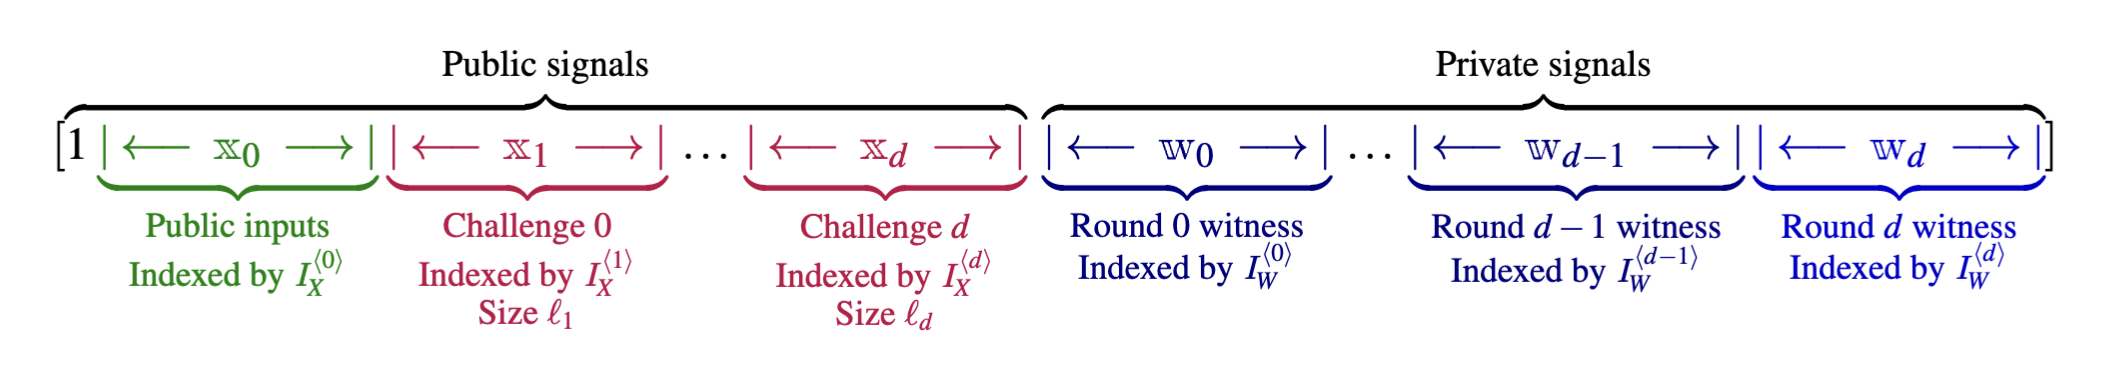
\includegraphics[width=1.0\textwidth]{images/lecture_18/wtns_structure.png}
        \end{figure}
    \end{frame}

    \begin{frame}{Strategy}
        \begin{definition}[Strategy]
            Define \textbf{strategy} for $\mathcal{R}_{\text{dQAP}}$ as the
            collection of functions $S=\{S_i\}_{i \in [d]}$ each of which
            computes the witness for the given round given previous witnesses
            and challenges and the current challenge, sampled by the verifier.
            In other words,
            \begin{equation*}
                \mathbbm{w}_i = S_i(\mathbbm{x}_0,\dots,\mathbbm{x}_i,\mathbbm{w}_0,\dots,\mathbbm{w}_{i-1})
            \end{equation*}
        \end{definition}

        \begin{example}
            0QAP represents the regular QAP with the strategy $S = \{S_0\}$ that
            consists of the witness generator: $\mathbbm{w} = S_0(\mathbbm{x})$.
            In turn, 1QAP represents the lookup Groth16 version where
            $\mathbbm{w}_0=S_0(\mathbbm{x}_0)$ computes the witness without
            lookups while
            $\mathbbm{w}_1=S_1(\mathbbm{x}_0,\mathbbm{x}_1,\mathbbm{w}_0)$
            computes lookup constraints.
        \end{example}
    \end{frame}

    \begin{frame}{$d$-round UltraGroth}
        Initialize accumulator $a_0 := \mathcal{H}(\sigma)$.

        \underline{\textbf{On each round $i \in [d]$:}}
        \begin{itemize}
            \item Sample $r_i \leftarrowS \mathbb{F}$.
            \item Compute witness $\mathbbm{w}_i \gets S_i(\mathbbm{x}_0,\dots,\mathbbm{x}_i,\mathbbm{w}_0,\dots,\mathbbm{w}_{i-1})$.
            \item Compute $\pi_C^{\langle i \rangle}$ with $c_i(X) :=
            \delta_i^{-1}\sum_{j \in \mathcal{I}_W^{\langle i \rangle}}
            z_j\zeta_j(X) + r_i\delta_d$.
            \item Update accumulator $a_{i+1} \gets \mathcal{H}(a_i, \pi_C^{\langle i \rangle})$.
            \item If $i<d$, for each $j \in \mathcal{I}_X^{\langle i+1 \rangle}$,
            set $z_j \gets \mathcal{H}(a_{i+1},g_1^j)$.
        \end{itemize}
    \end{frame}

    \begin{frame}{$d$-round UltraGroth: Last Round}
        \underline{\textbf{During the last round:}}
        \begin{itemize}
            \item Compute $h(X)$ similar to Groth16.
            \item Sample $r,s \leftarrowS \mathbb{F}$ and compute $\pi_A \gets
            g_1^{a(\tau)}$, $\pi_B \gets g_2^{b(\tau)}$, and the last proof
            piece $\pi_C^{\langle d \rangle} \gets g_1^{c_d(\tau)}$ where:
            \begin{gather*}
                a(X) = \alpha + \sum_{i \in [n]} z_i\ell_i(X) + r\delta_d, \; b(X) = \beta + \sum_{i \in [n]}z_ir_i(X) + s\delta_d, \\
                c_d(X) = \delta_d^{-1}\left(\sum_{i \in \mathcal{I}_W^{\langle d \rangle}}z_if_i(X) + h(X)t_{\Omega}(X)\right) + a(X)s+b(X)r-\sum_{i \in [d]}r_i\delta_i - rs\delta_d
            \end{gather*}
            \item \textbf{Output} proof $\pi = (\pi_A,\pi_B,\{\pi_C^{\langle i
            \rangle}\}_{i \in [d+1]}) \in \mathbb{G}_1 \times \mathbb{G}_2
            \times \mathbb{G}_1^{d+1}$. 
        \end{itemize}

        \underline{\textbf{Verification:}} $e(\pi_A,\pi_B) = e(g_1^{\alpha},g_2^{\beta}) \cdot e(g_1^{i(\tau)},g_2^{\gamma}) \cdot \prod_{i \in [d+1]}e(\pi_C^{\langle i \rangle}, g_2^{\delta_i})$.
    \end{frame}

    \begin{frame}{UltraGroth Efficiency}
    \textcolor{green!70!black}{\textbf{Groth16} performance} over
    the circuit of size $n$ and statement size $\ell$.
    \begin{itemize}
        \item \textbf{Prover work}: MSM of size $\mathcal{O}(n)$ over
        $\mathbb{G}_1$ and $\mathbb{G}_2$.
        \item \textbf{Proof size:} $2\mathbb{G}_1+\mathbb{G}_2$.
        \item \textbf{Verifier work:} 3 pairings + $\mathcal{O}(\ell)$
        $\mathbb{G}_1$ exps.
    \end{itemize}

    \textcolor{blue!70!black}{\textbf{UltraGroth} performance over $\mathcal{R}_{\text{dQAP}}$} in turn:
    \begin{itemize}
        \item \textbf{Prover work}: MSM of size
        $\mathcal{O}(\textcolor{blue!70!black}{n/\log n})$ over $\mathbb{G}_1$
        and $\mathbb{G}_2$.
        \item \textbf{Proof size:}
        $\textcolor{blue!70!black}{(d+2)}\mathbb{G}_1+\mathbb{G}_2$.
        \item \textbf{Verifier work:} \textcolor{blue!70!black}{$(d+3)$}
        pairings + $\mathcal{O}(\ell)$ $\mathbb{G}_1$ exps +
        \textcolor{blue!70!black}{$\sum_{i \in [d+1]\setminus
        \{0\}}|\mathbbm{x}_i|$ hashing operations}.
        \item Allowed interactiveness for potentially more complex protocols.
    \end{itemize}
    \end{frame}

    \begin{frame}[plain, standout]
        \centering
        \LARGE
        \textbf{Any Questions?} \\
        
        \vspace{0.2cm} \Huge \ding{170} \large \\
        
        \vspace{1cm}
  
        \href{https://zkdl-camp.github.io/}{\raisebox{-.1em}{\hspace{.025em}\faIcon{globe}}\hspace{.325em}zkdl-camp.github.io} \\
  
        \href{https://github.com/ZKDL-Camp}{\raisebox{-.1em}{\hspace{.025em}\faIcon{github}}\hspace{.325em}github.com/ZKDL-Camp}
        
        \begin{center}
            
\includegraphics[width=0.15\textwidth]{images/logo.png}
        \end{center}
    \end{frame}
\end{document}
